\documentclass[conference]{IEEEtran}
\IEEEoverridecommandlockouts
\usepackage{cite}
\usepackage{balance}
\usepackage{amsmath,amssymb,amsfonts}
\usepackage{graphicx}
\usepackage{textcomp}
\usepackage{xcolor}
\usepackage{booktabs}
\usepackage{tikz}
\usetikzlibrary{positioning,arrows.meta,fit,calc}
\usepackage[hidelinks]{hyperref}
\newcommand{\NTrainGauges}{193}
\newcommand{\NTestGauges}{48}
\newcommand{\NGauges}{242}
\newcommand{\AblMinutes}{3.4}
\newcommand{\NTrainRows}{1,641,197}
\newcommand{\NValRows}{349,645}
\newcommand{\NTestRows}{52,994}
\newcommand{\PosRate}{5.5}
\newcommand{\NFeat}{50}
\newcommand{\Thr}{0.45}
\newcommand{\GroupFlow}{11}
\newcommand{\GroupRain}{10}
\newcommand{\GroupWeather}{5}
\newcommand{\GroupSoil}{6}
\newcommand{\GroupSeason}{2}
\newcommand{\GroupStatic}{16}
\newcommand{\XgbBA}{0.898}
\newcommand{\XgbPR}{0.737}
\newcommand{\XgbRec}{0.902}
\newcommand{\XgbPrec}{0.328}
\newcommand{\XgbBALo}{0.886}
\newcommand{\XgbBAHi}{0.910}
\newcommand{\PersBA}{0.750}
\newcommand{\PersPR}{0.428}
\newcommand{\PersRec}{0.508}
\newcommand{\PersPrec}{0.789}
\newcommand{\PersBALo}{0.724}
\newcommand{\PersBAHi}{0.778}
\newcommand{\ClimBA}{0.802}
\newcommand{\ClimPR}{0.203}
\newcommand{\ClimRec}{0.891}
\newcommand{\ClimPrec}{0.152}
\newcommand{\ClimBALo}{0.774}
\newcommand{\ClimBAHi}{0.829}
\newcommand{\LstmBA}{0.873}
\newcommand{\LstmPR}{0.589}
\newcommand{\LstmRec}{0.826}
\newcommand{\LstmPrec}{0.376}
\newcommand{\LstmBALo}{0.829}
\newcommand{\LstmBAHi}{0.911}
\newcommand{\NoFlowBA}{0.853}
\newcommand{\NoFlowPR}{0.494}
\newcommand{\NoFlowRec}{0.865}
\newcommand{\NoFlowPrec}{0.239}
\newcommand{\NoFlowBALo}{0.820}
\newcommand{\NoFlowBAHi}{0.880}
\newcommand{\DiffPersLo}{0.123}
\newcommand{\DiffPersHi}{0.175}
\newcommand{\LstmCov}{100}
\newcommand{\LstmCompare}{On the rows it covers, the model (0.898) and the simulation (0.873) were statistically indistinguishable in balanced accuracy, although only the model is a real forecast.}
\newcommand{\AblAllBA}{0.898}
\newcommand{\AblAllPR}{0.736}
\newcommand{\AlarmsThr}{150}
\newcommand{\PrecSeventyFive}{0.539}
\newcommand{\RecSeventyFive}{0.760}
\newcommand{\EceRaw}{0.102}
\newcommand{\EceIso}{0.005}
\newcommand{\CalWord}{over-confident}
\newcommand{\PgN}{46}
\newcommand{\PgMed}{0.900}
\newcommand{\PgQOne}{0.860}
\newcommand{\PgQThree}{0.926}
\newcommand{\PgMin}{0.769}
\newcommand{\EvN}{266}
\newcommand{\EvXgbWarn}{91.4}
\newcommand{\EvLstmWarn}{83.5}
\newcommand{\EvClimWarn}{89.5}
\newcommand{\EvPersWarn}{0.0}
\newcommand{\EvNoFlowWarn}{94.0}
\newcommand{\LeakRandBA}{0.915}
\newcommand{\LeakRandPR}{0.810}
\newcommand{\LeakTimeBA}{0.892}
\newcommand{\LeakTimePR}{0.724}
\newcommand{\LeakSpaceBA}{0.905}
\newcommand{\LeakSpacePR}{0.789}
\newcommand{\LeakSpTiBA}{0.898}
\newcommand{\LeakSpTiPR}{0.736}
\newcommand{\LeakGapBA}{1.7}
\newcommand{\LeakGapPR}{7.4}
\newcommand{\LeakText}{The random row split gave the highest balanced accuracy, 0.915, against 0.898 on unseen gauges in later years. Its test rows were 1.7 points higher in balanced accuracy and 7.4 points higher in PR-AUC, but the bootstrap intervals barely separate and the two test sets differ in gauges, years and flood rate, so the gap is indicative rather than tested. PR-AUC ranged from 0.724 (new years) to 0.810 (random rows). Holding out later years lowered PR-AUC more than holding out gauges (0.724 against 0.789), which suggests that a temporal split matters at least as much as a spatial one. In the spatial protocol, the test years are also the years from which each gauge's flood threshold was computed. Flood prevalence differs between protocols (7.4\% of random rows against 5.5\% in the held-out test), which moves PR-AUC on its own.}
\newcommand{\LeakDiscuss}{a random row split scored 1.7 points higher in balanced accuracy on its own test rows (Table~\ref{tab:leak}); the test sets differ, so the gap is indicative, but it points the same way as the literature, and published Indian flood models can only be compared under the same split.}
\newcommand{\LeakConclude}{A random row split scored 1.7 points higher on its own, different test rows, so the split should be reported with every score.}
\newcommand{\LeakAbstract}{Retrained on a random row split, the same configuration scored 0.915 on its own test rows, an indicative gap of 1.7 points.}
\newcommand{\LeadOne}{96.7}
\newcommand{\LeadOneRise}{90.3}
\newcommand{\LeadTwo}{93.3}
\newcommand{\LeadTwoRise}{85.2}
\newcommand{\LeadThree}{89.5}
\newcommand{\LeadThreeRise}{80.0}
\newcommand{\FpMonsoonPct}{86}
\newcommand{\MonPrec}{0.311}
\newcommand{\OthPrec}{0.415}
\newcommand{\MonAlarms}{372}
\newcommand{\OthAlarms}{36}
\newcommand{\NearMissMon}{21}
\newcommand{\FaRatioMon}{41}
\newcommand{\PgGauges}{46}
\newcommand{\RhoArea}{0.44}
\newcommand{\PArea}{0.002}
\newcommand{\PMinOther}{0.64}
\newcommand{\WarnThreeXgb}{63.9}
\newcommand{\WarnThreeLstm}{78.9}
\newcommand{\WarnThreeClim}{89.1}
\newcommand{\EvGauges}{44}
\newcommand{\MeanLeadXgb}{2.58}
\newcommand{\ImpFlow}{67.5}
\newcommand{\ImpRain}{13.6}
\newcommand{\ImpWeather}{7.3}
\newcommand{\ImpTopOne}{40.5}
\newcommand{\ImpTopTwo}{23.9}
\newcommand{\ImpRainDay}{8.5}
\newcommand{\RelHiConf}{0.97}
\newcommand{\RelHiFreq}{0.75}
\newcommand{\OnsetAll}{0.852}
\newcommand{\OnsetNoFlow}{0.846}
\newcommand{\OnsetFlowOnly}{0.810}
\newcommand{\AblOnTol}{0.006}
\newcommand{\OnXgbBA}{0.857}
\newcommand{\OnXgbPR}{0.369}
\newcommand{\OnLstmBA}{0.877}
\newcommand{\OnLstmPR}{0.421}
\newcommand{\OnTrendBA}{0.734}
\newcommand{\OnTrendPR}{0.158}
\newcommand{\OnClimBA}{0.802}
\newcommand{\OnClimPR}{0.102}
\newcommand{\OnPersBA}{0.500}
\newcommand{\OnPersPR}{0.026}
\newcommand{\TrendBA}{0.828}
\newcommand{\TrendPR}{0.605}
\newcommand{\XgbCSI}{0.317}
\newcommand{\LstmCSI}{0.349}
\newcommand{\TrendCSI}{0.277}
\newcommand{\ClimCSI}{0.149}
\newcommand{\PersCSI}{0.448}
\newcommand{\XgbFAR}{0.672}
\newcommand{\MonN}{17,992}
\newcommand{\OthN}{35,002}
\newcommand{\CsiSeventyFive}{0.461}
\newcommand{\LstmDiffLo}{-0.009}
\newcommand{\LstmDiffHi}{0.063}
\newcommand{\LstmDiffOnLo}{-0.045}
\newcommand{\LstmDiffOnHi}{0.011}
\newcommand{\LstmAlarm}{120}
\newcommand{\MatchPrec}{0.394}
\newcommand{\MatchRec}{0.864}
\newcommand{\UnseenNoRows}{1}
\newcommand{\NUnseen}{49}
\newcommand{\SeenTestGauges}{181}
\newcommand{\BrierRaw}{0.065}
\newcommand{\BrierIso}{0.025}
\newcommand{\BrierClim}{0.048}
\newcommand{\EceRawLo}{0.094}
\newcommand{\EceRawHi}{0.110}
\newcommand{\EceIsoLo}{0.002}
\newcommand{\EceIsoHi}{0.008}
\newcommand{\EceMonRaw}{0.250}
\newcommand{\EceMonIso}{0.014}
\newcommand{\EceOthRaw}{0.026}
\newcommand{\YearMinBA}{0.873}
\newcommand{\YearMaxBA}{0.914}
\newcommand{\YearMin}{2017}
\newcommand{\YearMax}{2016}
\newcommand{\YearsBig}{2015--2018}
\newcommand{\YearsSmallRows}{2,102}
\newcommand{\YearsSmall}{2019 and 2020}
\newcommand{\YearLateBA}{0.783 in 2019 and 0.767 in 2020}
\newcommand{\RegRho}{0.37}
\newcommand{\RegP}{0.02}
\newcommand{\RegRhoRes}{0.20}
\newcommand{\RegPRes}{0.23}
\newcommand{\RegDams}{37}
\newcommand{\RegNoDams}{9}
\newcommand{\RegBADams}{0.911}
\newcommand{\RegBANoDams}{0.875}
\newcommand{\NsTrain}{5.0}
\newcommand{\NsTest}{3.9}
\newcommand{\DropN}{281,360}
\newcommand{\DropPct}{9.3}
\newcommand{\DropMon}{26}
\newcommand{\KeptMon}{34}
\newcommand{\DropHigh}{1.5}
\newcommand{\KeptHigh}{4.9}
\newcommand{\EpN}{1,441}
\newcommand{\EpFalse}{1,106}
\newcommand{\EpFalsePct}{77}
\newcommand{\RandWarn}{38.6}
\newcommand{\RandWarnMon}{75.2}
\newcommand{\SplitN}{5}
\newcommand{\SplitBAMin}{0.877}
\newcommand{\SplitBAMax}{0.898}
\newcommand{\SplitPRMin}{0.706}
\newcommand{\SplitPRMax}{0.764}
\newcommand{\SplitOnMin}{0.822}
\newcommand{\SplitOnMax}{0.851}
\newcommand{\SplitBAMean}{0.889}
\newcommand{\SplitBASd}{0.008}
\newcommand{\BasinN}{5}
\newcommand{\BasinCount}{15}
\newcommand{\BasinOnMin}{0.785}
\newcommand{\BasinOnMax}{0.864}
\newcommand{\BasinWorst}{Cauvery, EFRN, EFRS, Tapi}
\newcommand{\BasinBAMin}{0.866}
\newcommand{\BasinBAMax}{0.906}
\newcommand{\BasinPRMin}{0.648}
\newcommand{\BasinPRMax}{0.829}
\newcommand{\MetBA}{0.832}
\newcommand{\MetOnBA}{0.825}
\newcommand{\MetPR}{0.447}
\newcommand{\QnnBA}{0.853}
\newcommand{\QnnPR}{0.364}
\newcommand{\QnnPrev}{1.6}
\newcommand{\QnnPrec}{0.117}
\newcommand{\QnnOnBA}{0.798}
\newcommand{\NcwEce}{0.008}
\newcommand{\NcwBA}{0.902}
\newcommand{\NcwText}{When the model was refit without the positive-class weight, its raw ECE was 0.008, so the weighting explains most of the over-confidence.}
\newcommand{\CandLrBA}{0.899}
\newcommand{\CandLrPR}{0.751}
\newcommand{\CandSelBA}{0.911}
\newcommand{\CandSelPR}{0.796}
\newcommand{\CandGainPR}{4.5}
\newcommand{\MainBAGYLo}{0.870}
\newcommand{\MainBAGYHi}{0.916}
\newcommand{\BelNoFlowDiff}{0.007}
\newcommand{\BelNoFlowLo}{-0.005}
\newcommand{\BelNoFlowHi}{0.020}
\newcommand{\BelNoMetDiff}{0.042}
\newcommand{\BelNoMetLo}{0.025}
\newcommand{\BelNoMetHi}{0.061}
\newcommand{\BelMetFlowDiff}{0.015}
\newcommand{\BelMetFlowLo}{-0.006}
\newcommand{\BelMetFlowHi}{0.039}
\newcommand{\MatchAlarms}{144}
\newcommand{\MatchWarnAll}{89.5}
\newcommand{\MatchWarnNoFlow}{88.7}
\newcommand{\OwnWarnNoFlow}{94.0}
\newcommand{\NoFlowAlarms}{197}
\newcommand{\ClimCorrMin}{0.97}
\newcommand{\ClimTrBA}{0.897}
\newcommand{\ClimTrPR}{0.737}
\newcommand{\ClimTrBelow}{0.855}
\newcommand{\ClimTrLo}{-0.001}
\newcommand{\ClimTrHi}{0.004}
\newcommand{\NoClimBA}{0.896}
\newcommand{\NoClimPR}{0.729}
\newcommand{\NoClimBelow}{0.854}
\newcommand{\NoClimLo}{-0.001}
\newcommand{\NoClimHi}{0.006}
\newcommand{\RtBA}{0.893}
\newcommand{\RtPR}{0.721}
\newcommand{\RtBelow}{0.844}
\newcommand{\RtLo}{0.000}
\newcommand{\RtHi}{0.011}
\newcommand{\RtDiff}{0.005}
\newcommand{\RtBelLo}{-0.003}
\newcommand{\RtBelHi}{0.019}
\newcommand{\LrTestBA}{0.893}
\newcommand{\LrTestPR}{0.682}
\newcommand{\LrDiffLo}{0.000}
\newcommand{\LrDiffHi}{0.010}
\newcommand{\LrGainPR}{5.4}
\newcommand{\RtLate}{humidity, evapotranspiration and soil moisture}
\newcommand{\SrN}{10,793}
\newcommand{\SrGauges}{48}
\newcommand{\SrRandBA}{0.925}
\newcommand{\SrHeldBA}{0.906}
\newcommand{\SrRandPR}{0.803}
\newcommand{\SrHeldPR}{0.771}
\newcommand{\SrBALo}{1.2}
\newcommand{\SrBAHi}{2.5}
\newcommand{\SrPRLo}{1.8}
\newcommand{\SrPRHi}{4.7}
\newcommand{\SrGapBA}{1.8}
\newcommand{\SrGapPR}{3.2}
\newcommand{\McCSI}{0.490}
\newcommand{\McPrec}{0.671}
\newcommand{\McRec}{0.645}
\newcommand{\McAlarms}{52}
\newcommand{\McWarn}{54}
\newcommand{\HyCSI}{0.500}
\newcommand{\HyPrec}{0.658}
\newcommand{\HyRec}{0.677}
\newcommand{\HyAlarms}{56}
\newcommand{\HyWarn}{54}
\newcommand{\PeCSI}{0.448}
\newcommand{\PePrec}{0.789}
\newcommand{\PeRec}{0.508}
\newcommand{\PeAlarms}{35}
\newcommand{\PeWarn}{0}
\newcommand{\MbCSI}{0.317}
\newcommand{\MbPrec}{0.328}
\newcommand{\MbRec}{0.902}
\newcommand{\MbAlarms}{150}
\newcommand{\MbWarn}{91}
\newcommand{\HyThr}{0.86}
\newcommand{\McThr}{0.86}
\newcommand{\HyMLo}{0.004}
\newcommand{\HyMHi}{0.020}
\newcommand{\HyPLo}{0.032}
\newcommand{\HyPHi}{0.073}
\newcommand{\McPLo}{0.019}
\newcommand{\McPHi}{0.065}
\newcommand{\TradeMax}{0.424}
\newcommand{\MlpBA}{0.862}
\newcommand{\MlpPR}{0.596}
\newcommand{\MlpBelow}{0.822}
\newcommand{\MlpWin}{14}
\newcommand{\MlpDiffLo}{0.023}
\newcommand{\MlpDiffHi}{0.050}


\begin{document}

\title{When Random Splits Flatter Flood Forecasts: Three-Day High-Flow Warnings at Held-Out Indian Gauges}

\author{\IEEEauthorblockN{Anonymous Author(s)}
\IEEEauthorblockA{\textit{Affiliation withheld for double-blind review}}}

\maketitle

\begin{abstract}
Machine-learning flood forecasters are often scored on random row splits, which let neighbouring days of the same river leak between training and test data. We build a leakage-controlled benchmark on CAMELS-IND for one question: will a gauge's flow exceed its 95th-percentile level within three days? We train on \NTrainGauges{} gauges in 1980--2008, select on 2009--2014 and test once on \NTestGauges{} held-out gauges in 2015--2020; each test gauge still needs its own 1980--2008 record and a flow reading on the forecast day. Averaged over six gauge splits, a gradient-boosted model reached a balanced accuracy (BA) of \SplitBAMean; on the primary split it reached \XgbBA{} (gauge-and-year bootstrap interval \MainBAGYLo--\MainBAGYHi), against \PersBA{} for persistence. Scored on the same rows, a model trained on a random row split was \SrGapBA{} BA points higher (interval \SrBALo--\SrBAHi), so random splits overstate skill at new gauges. Recomputing the climate indices from training years only made no detectable difference, and restricting the model to inputs available in real time lowered BA by only \RtDiff. At the BA threshold, precision was only \XgbPrec{} and persistence had the higher critical success index (CSI); a rule that keeps persistence for rivers already above the level and uses the model elsewhere, set on validation, raised CSI to \HyCSI{} against \PeCSI, at the cost of fewer onset warnings.
\end{abstract}

\begin{IEEEkeywords}
CAMELS-IND, data leakage, early warning, flood forecasting, gradient boosting, streamflow
\end{IEEEkeywords}

\section{Introduction}
An emergency officer watching an Indian river gauge needs a plain answer: is the flow likely to reach its flood level in the next few days? Machine-learning models trained on many catchments now simulate streamflow well, even in basins without a gauge record \cite{Kratzert2019a,Kratzert2019b,Nearing2024}. Reported skill, however, depends on how a model is evaluated. When rows are split at random, days from the same flood fall on both sides of the split, and part of the test score then rewards memory of the event \cite{Kapoor2023,Roberts2017}.

India now has a large-sample dataset to study this properly. CAMELS-IND provides daily forcing, observed streamflow and catchment attributes for peninsular Indian catchments \cite{Mangukiya2025}, in the format of the CAMELS family \cite{Newman2015,Addor2017}. It also ships a regional long short-term memory (LSTM) simulation of streamflow, which gives a strong deep-learning reference at no extra cost. What is missing is a short-range flood-exceedance benchmark on these gauges that controls leakage, compares against simple and strong references, and reports the numbers an operations room needs: alarm rates, onset lead time and calibration.

We build such a benchmark. The classifier is a standard gradient-boosted model; what is new is the task, the split and what they show:
\begin{enumerate}
\item A leakage-controlled exceedance benchmark on CAMELS-IND: gauges held out in space and time, thresholds and model choices from training and validation years only, repeated gauge splits and leave-basin-out folds, and a same-rows measurement of how much a random row split inflates the score (Fig.~\ref{fig:split}).
\item A feature-group ablation with paired gauge-bootstrap intervals, and comparisons with persistence, a trend rule, climatology and the CAMELS-IND LSTM. Today's flow carries most of the overall score; on rivers still below their level, removing the flow inputs made no detectable difference, while removing all the other inputs together did.
\item An operational evaluation: skill on below-level rows, alarms per 1,000 gauge-days, alarm episodes, calibration, a fallback that needs no flow reading, and a persistence-gated decision rule, chosen on validation, that beats persistence on the critical success index (CSI).
\end{enumerate}

\section{Related Work}
\textit{Large-sample learning.} The CAMELS datasets standardised forcing, flow and attributes across hundreds of basins \cite{Newman2015,Addor2017}. LSTMs trained on them learn regional behaviour \cite{Kratzert2019a}, predict ungauged basins \cite{Kratzert2019b}, simulate extremes well \cite{Frame2022} and forecast extreme floods globally \cite{Nearing2024}; river-network graphs have not yet beaten them \cite{Kirschstein2024}. Most of this work simulates streamflow, and the exceedance on which warnings are issued is derived afterwards.

\textit{Operational forecasting.} Physically based ensemble systems such as GloFAS \cite{Alfieri2013} dominate operational forecasting \cite{Cloke2009}, and a learned system now forecasts river stage for India and Bangladesh \cite{Nevo2022}. INDOFLOODS catalogues Indian flood events \cite{Kuntla2025}, and many studies fit tree ensembles or neural networks to single basins \cite{Mosavi2018}.

\textit{Evaluation.} Leakage through the split is a leading cause of irreproducible machine-learning results \cite{Kapoor2023}, and data with spatial or temporal structure need blocked validation \cite{Roberts2017}. For rare events, precision--recall curves are more informative than ROC curves \cite{Saito2015}, and probabilistic forecasts should be checked for calibration \cite{Brier1950}.

Earlier studies held out basins for daily flow in the USA \cite{Kratzert2019b} or for flood events globally \cite{Nearing2024}, held out time in Europe \cite{Kirschstein2024}, or released CAMELS-IND with a regional LSTM but no exceedance task \cite{Mangukiya2025}. To our knowledge, no study has benchmarked short-range flood-exceedance forecasting on CAMELS-IND with a space-and-time held-out split against both a learned streamflow simulation and simple references.

\section{Data and Task}
\subsection{Target}
For gauge $g$ on day $t$ the target is
\begin{equation}
y_{g,t}=\mathbb{1}\Big[\max_{h\in\{1,2,3\}} Q_{g,t+h}\ \ge\ q^{95}_g\Big],
\label{eq:target}
\end{equation}
where $Q$ is observed streamflow and $q^{95}_g$ is the 95th percentile of the gauge's flow over the training years 1980--2008 only. A day with $y_{g,t}=1$ is a \emph{flood window}. The level is a statistical proxy, exceeded on one day in twenty in the training years; CAMELS-IND gives no official danger levels, and a stricter 99th-percentile level is tested in Section~\ref{sec:robust}. We assume that three days is enough to stage rescue teams; we did not survey operators. Days with no flow observation on any of $t{+}1$ to $t{+}3$ are dropped, and when only some are observed the maximum is taken over those, which can miss an exceedance on a missing day. The \DropN{} dropped gauge-days (\DropPct\%) were not concentrated in the monsoon (\DropMon\% against \KeptMon\% of kept days) or after high flow.

\subsection{Inputs}
The \NFeat{} inputs, all known at the end of day $t$, are \GroupFlow{} streamflow features (lags of 0--3 days, 1- and 3-day changes, 7- and 30-day means, 7-day maximum, log flow and a reading flag), \GroupRain{} rainfall features (lags, 3- to 90-day sums, 7-day maximum), \GroupWeather{} weather and \GroupSoil{} soil-moisture inputs, \GroupSeason{} for the season and \GroupStatic{} catchment attributes (area, slope, climate indices, land cover, soils). All flow features except one log-flow input are scaled by $q^{95}_g$, so they read as ``how close the river is to its flood level''. Hydrological signatures of CAMELS-IND are excluded, because they are computed over the full 1980--2020 record and would leak test-period information; future rainfall is excluded as well. The four CAMELS-IND climate indices we keep (mean rainfall and evapotranspiration, aridity, high-rainfall frequency) are computed over the dataset period, which includes our test years; recomputed from 1980--2008 forcing only, they gave the same skill (Section~\ref{sec:robust}). Rainfall is the gridded product of the India Meteorological Department (IMD); soil moisture, humidity and evapotranspiration come from the Indian Monsoon Data Assimilation and Analysis (IMDAA) reanalysis and the Global Land Evaporation Amsterdam Model (GLEAM) \cite{Mangukiya2025}. These products are released with a delay, so Section~\ref{sec:robust} also tests the model without them.

\subsection{Split}
Fig.~\ref{fig:split} shows the split. All \NGauges{} gauges in the observed-streamflow file have forcing data and at least three years of flow in 1980--2008, so none is excluded; the dataset paper describes 228 catchments \cite{Mangukiya2025}, while the streamflow file we use lists \NGauges, all with more than 30\% flow availability. This is not an ungauged-basin method: each test gauge needs its 1980--2008 record for the flood level, climatology and flow scaling, and a flow reading on day $t$; ``unseen'' means unseen in training. A group split puts 20\% of gauges aside (seed 42), so the primary test asks about rivers the model has never seen, in years it has never seen; of the \NUnseen{} unseen gauges, \UnseenNoRows{} gauge has no flow record in 2015--2020, which leaves \NTestGauges{} test gauges. Training uses the other gauges in 1980--2008 (\NTrainRows{} gauge-days), validation the same gauges in 2009--2014 (\NValRows), and the test the unseen gauges in 2015--2020, all labelled by (\ref{eq:target}) (\NTestRows{} gauge-days, of which \PosRate\% are flood windows).

\begin{figure}[t]
\centering
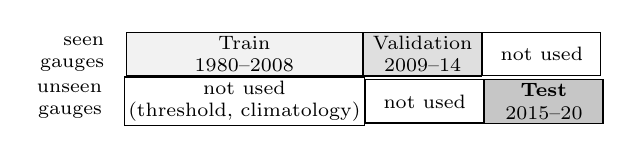
\begin{tikzpicture}[font=\scriptsize,
  cell/.style={draw, minimum height=0.55cm, align=center, inner sep=1.5pt},
  arr/.style={-{Latex[length=1.4mm]}, semithick}]
\node[cell, minimum width=3.0cm, fill=gray!10] (tr) at (0,0) {Train\\1980--2008};
\node[cell, minimum width=1.5cm, fill=gray!25, right=0pt of tr] (va) {Validation\\2009--14};
\node[cell, minimum width=1.5cm, right=0pt of va] (sx) {not used};
\node[cell, minimum width=3.0cm, below=0pt of tr] (ux) {not used\\(threshold, climatology)};
\node[cell, minimum width=1.5cm, right=0pt of ux] (uy) {not used};
\node[cell, minimum width=1.5cm, fill=gray!45, right=0pt of uy] (te) {\textbf{Test}\\2015--20};
\node[left=0.15cm of tr, align=right] {seen\\gauges};
\node[left=0.15cm of ux, align=right] {unseen\\gauges};
\end{tikzpicture}
\caption{Leakage-controlled split. The primary test uses gauges and years that played no part in training, model selection or threshold choice. The unseen gauges' 1980--2008 record is used only to set their flood level and climatology.}
\label{fig:split}
\end{figure}

\section{Methods}
\textit{Model.} Seven candidates (logistic regression, random forest, histogram gradient boosting and four XGBoost \cite{Chen2016} configurations) were compared on validation balanced accuracy, and the decision threshold of the selected depth-6 XGBoost model, \Thr, was set on validation as well. The selected model uses a learning rate of 0.05, subsampling of rows and columns at 0.8, a minimum child weight of 20, L2 regularisation of 5 and a positive-class weight equal to the ratio of negative to positive training rows. Training stops early on the validation area under the precision--recall curve (PR-AUC). The candidates were fitted on one 500,000-row training sample; the depth-6 configuration was then refit on all training rows and kept because it scored higher on validation. In validation balanced accuracy all seven lay between \CandLrBA{} (logistic regression) and \CandSelBA{} (the selected model). The sample-fitted model had been scored on the test set during development, before this refit; no choice of model, input or threshold used that score, and the later six-split and basin-fold results agree. Balanced accuracy is $\mathrm{BA}=(\mathrm{TPR}+\mathrm{TNR})/2$, the mean of the true positive and true negative rates.

\textit{References.} \emph{Persistence} forecasts a flood window if the river is above its flood level today, and no flood on a day without a reading. A \emph{trend rule} needs no learning: its score is $Q_{g,t}/q^{95}_g+\max(0,Q_{g,t}-Q_{g,t-3})/q^{95}_g$, so a high or rising river raises an alarm. \emph{Climatology} forecasts the gauge's own 1980--2008 rate of flood windows within $\pm15$ days of the calendar day. The \emph{LSTM simulation} is the regional LSTM streamflow of CAMELS-IND \cite{Mangukiya2025}, scored as $\max_{h\le3}\hat Q_{g,t+h}/q^{95}_g$. It is driven by observed forcing, so it sees the rain of days $t{+}1$ to $t{+}3$, which no real forecast has. It was trained by the dataset authors on 159 catchments over 1991--2015 and tested on 2016--2020 \cite{Mangukiya2025}, so it has most likely seen our test gauges and, in 2015, one of our test years. It is therefore an optimistic reference, not a held-out competitor. Thresholds of the references were set on validation like the model's.

\textit{Analyses.} We refit the selected configuration on the same 500,000-row training sample with one input group removed at a time, and with only the streamflow and season inputs or only the meteorological and season inputs. Percentile intervals come from 1,000 resamples of the test gauges (500 for the protocol comparison and the ECE), which keeps each river's days together; the main score also gets a gauge-by-year resample, because the test covers few years. Calibration is the expected calibration error (ECE) \cite{Naeini2015} over ten bins, before and after isotonic regression fitted on the validation years of the seen gauges and applied unchanged to the unseen test gauges. A flood onset is a day on which the river reaches $q^{95}_g$ after at least seven days below it; a method warns of it if it forecasts a flood window one, two or three days earlier. The monsoon is June to September. Robustness refits (Section~\ref{sec:robust}) use the ablation's 500,000-row sample. They cover five more random gauge splits (seeds 1 to 5), a leave-basin-out evaluation and the same task with the 99th percentile as the level. For leave-basin-out, the CAMELS-IND river basins are grouped into five folds, and every basin is held out once and tested on 2015--2020.

\textit{Reproducibility.} Splits and resamples use seed 42; code, model and the list of held-out gauges are available from the authors (link withheld for review), and every number here is generated from the experiment outputs by a script that checks each claim.

\section{Results}
\subsection{Skill on Unseen Gauges}
Table~\ref{tab:main} and Fig.~\ref{fig:pr} give the main comparison. The model scored above persistence and climatology in balanced accuracy, recall and PR-AUC, and its interval for the gain over persistence (\DiffPersLo--\DiffPersHi) excludes zero. Resampling test years as well as gauges widened the interval of its balanced accuracy to \MainBAGYLo--\MainBAGYHi. Persistence was more precise (\PersPrec{} against \XgbPrec) because a river already above its level usually stays there, but it misses every flood that has not yet begun. On below-level rows, where the river is still below the level, the model reached a balanced accuracy of \OnXgbBA{} and a PR-AUC of \OnXgbPR, above the trend rule, climatology and persistence. On the critical success index, $\mathrm{CSI}=\mathrm{TP}/(\mathrm{TP}+\mathrm{FP}+\mathrm{FN})$ \cite{Jolliffe2012}, which ignores correct negatives, persistence scored highest at this threshold (\PersCSI, against \XgbCSI{} for the model); Section~\ref{sec:rules} returns to this.

\begin{table}[t]
\caption{Three-day exceedance on \NTestGauges{} unseen gauges, 2015--2020}
\label{tab:main}
\centering
\footnotesize
\setlength{\tabcolsep}{1.7pt}
\begin{tabular}{lccccccc}
\toprule
 & \multicolumn{6}{c}{all rows} & below-\\
Method & BA & 95\% CI & PR-AUC & Rec. & Prec. & CSI & level BA\\
\midrule
XGBoost (ours) & 0.898 & 0.886--0.910 & 0.737 & 0.902 & 0.328 & 0.317 & 0.857\\
No-flow XGB.$^\ddagger$ & 0.853 & 0.820--0.880 & 0.494 & 0.865 & 0.239 & 0.230 & 0.846\\
LSTM sim.$^\dagger$ & 0.873 & 0.829--0.911 & 0.589 & 0.826 & 0.376 & 0.349 & 0.877\\
Trend rule & 0.828 & 0.811--0.845 & 0.605 & 0.754 & 0.305 & 0.277 & 0.734\\
Climatology & 0.802 & 0.774--0.829 & 0.203 & 0.891 & 0.152 & 0.149 & 0.802\\
Persistence & 0.750 & 0.724--0.778 & 0.428 & 0.508 & 0.789 & 0.448 & 0.500\\
\bottomrule
\multicolumn{8}{l}{\scriptsize CI: 95\% gauge bootstrap. Below-level: river below $q^{95}_g$ on day $t$.}\\
\multicolumn{8}{l}{\scriptsize $^\dagger$Sees observed future rain. $^\ddagger$500,000-row refit (Table~\ref{tab:abl}).}\\
\end{tabular}
\end{table}

\begin{figure}[t]
\centering
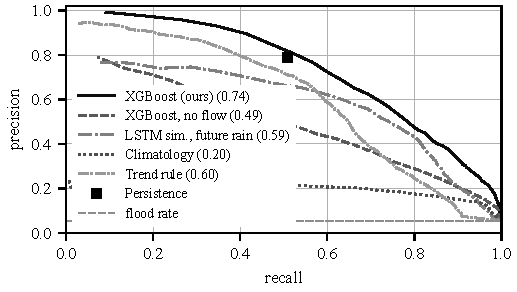
\includegraphics[width=\columnwidth]{fig_pr.pdf}
\caption{Precision--recall curves on the unseen test gauges; PR-AUC in brackets. The square is persistence, a single operating point; the flat line is the flood rate, the level of no skill.}
\label{fig:pr}
\end{figure}

The LSTM simulation is a demanding reference because it knows the rain that is still to fall. Over all rows its balanced accuracy was \LstmBA{} against \XgbBA{} for the model, and the paired gauge-bootstrap interval of the difference, \LstmDiffLo{} to \LstmDiffHi, includes zero. On below-level rows the LSTM scored higher (\OnLstmBA{} against \OnXgbBA), as its access to future rain would suggest, yet this gap was also within sampling noise (interval \LstmDiffOnLo{} to \LstmDiffOnHi).

\subsection{Effect of the Evaluation Protocol}
To see what the split alone does, we trained the same configuration under four protocols, each with its own validation set, and scored each once (Table~\ref{tab:leak}). The random row split scored highest, but its test set differs from ours in gauges, years and flood rate. We therefore also scored it and the held-out model on the same \SrN{} rows: random-split test rows that belong to held-out gauges in 2015--2020. On these shared rows the random split was \SrGapBA{} points higher in balanced accuracy (interval \SrBALo--\SrBAHi) and \SrGapPR{} points higher in PR-AUC (\SrPRLo--\SrPRHi). It had trained on other days of the same rivers and years, the most likely reason. Holding out later years lowered PR-AUC more than holding out gauges, which suggests that a temporal split matters at least as much as a spatial one, although flood rates differ between those test sets.

\begin{table}[t]
\caption{Same configuration, four protocols (500,000-row refit)}
\label{tab:leak}
\centering
\footnotesize
\setlength{\tabcolsep}{1.6pt}
\begin{tabular}{lcccccc}
\toprule
Test set & Gauges & Flood \% & BA & 95\% CI & PR-AUC & Prec.\\
\midrule
Random rows & 242 & 7.4 & 0.915 & 0.911--0.919 & 0.810 & 0.426\\
New years & 181 & 6.1 & 0.892 & 0.885--0.898 & 0.724 & 0.349\\
New gauges & 49 & 7.6 & 0.905 & 0.898--0.912 & 0.789 & 0.424\\
New gauges + years & 48 & 5.5 & 0.898 & 0.886--0.911 & 0.736 & 0.340\\
\bottomrule
\multicolumn{7}{l}{\scriptsize Random: 70/10/20\% of gauge-days. Others: trained on seen}\\
\multicolumn{7}{l}{\scriptsize gauges, 1980--2008; new years: seen gauges with flow in 2015--20; new}\\
\multicolumn{7}{l}{\scriptsize gauges: unseen, 1980--2008 (threshold years). CIs rounded; at}\\
\multicolumn{7}{l}{\scriptsize four decimals the first and last do not overlap.}\\
\end{tabular}
\end{table}

\subsection{What the Forecast Relies On}
Over all rows, removing the streamflow inputs cost the most in the ablation (Table~\ref{tab:abl}), lowering balanced accuracy from \AblAllBA{} to \NoFlowBA{} and PR-AUC from \AblAllPR{} to \NoFlowPR, while removing soil moisture, rainfall or catchment attributes cost little. On below-level rows the picture changes. Without streamflow the below-level balanced accuracy fell only from \OnsetAll{} to \OnsetNoFlow{} (paired difference \BelNoFlowLo{} to \BelNoFlowHi), whereas streamflow and season alone reached \OnsetFlowOnly{} (difference \BelNoMetLo{} to \BelNoMetHi) and meteorology and season alone \MetOnBA. For rivers still below their level, then, the non-flow inputs carried the skill and the flow inputs added little, although neither group alone matched the full model. The non-flow groups overlap: removing rainfall, soil moisture or catchment attributes one at a time changed below-level balanced accuracy by less than \AblOnTol, so these single-group results cannot rank them. The no-flow variant also scored above climatology overall (\NoFlowBA{} against \ClimBA), so it is a usable fallback when a gauge reading is missing.

\begin{table}[t]
\caption{Feature-group ablation (500,000-row training sample)}
\label{tab:abl}
\centering
\footnotesize
\setlength{\tabcolsep}{3pt}
\begin{tabular}{lccccc}
\toprule
Inputs & $n$ & BA & PR-AUC & Rec. & Below-level BA\\
\midrule
All inputs & 50 & 0.898 & 0.736 & 0.897 & 0.852\\
No streamflow & 39 & 0.853 & 0.494 & 0.865 & 0.846\\
No catchment & 34 & 0.895 & 0.734 & 0.907 & 0.855\\
No soil moisture & 44 & 0.896 & 0.732 & 0.895 & 0.854\\
No rainfall & 40 & 0.897 & 0.730 & 0.901 & 0.857\\
Streamflow + season & 13 & 0.875 & 0.685 & 0.882 & 0.810\\
Meteorology + season & 23 & 0.832 & 0.447 & 0.833 & 0.825\\
\bottomrule
\multicolumn{6}{l}{\scriptsize Below-level BA: rows where the river is below its flood level on day $t$.}\\
\end{tabular}
\end{table}

\subsection{Robustness}
\label{sec:robust}
Table~\ref{tab:robust} repeats the evaluation with refits that are directly comparable with each other. The primary split sits at the top of the range over six gauge splits, so its scores are, if anything, optimistic; averaged over all six, balanced accuracy was \SplitBAMean{} (s.d.\ \SplitBASd). Whole river basins held out gave \BasinBAMin--\BasinBAMax, so gauges on the same river as a training gauge did not carry the result. With the stricter 99th-percentile level, only \QnnPrev\% of test rows were positive and balanced accuracy fell to \QnnBA. By year, skill was steady over \YearsBig{} but lower in the sparse late years (\YearLateBA).

The inputs passed three checks. Climate indices recomputed from training years only, or dropped altogether, made no detectable difference. Dropping the late-arriving reanalysis inputs (\RtLate) lowered balanced accuracy by only \RtDiff{} (interval \RtLo--\RtHi) and below-level skill by no detectable amount. Two other learners did worse on the same sample: logistic regression came close in balanced accuracy but trailed by \LrGainPR{} points of PR-AUC, and a neural network (a multilayer perceptron with a \MlpWin-day input history) reached \MlpBA, below the model by \MlpDiffLo--\MlpDiffHi.

\begin{table}[t]
\caption{Robustness refits (500,000-row training sample)}
\label{tab:robust}
\centering
\footnotesize
\setlength{\tabcolsep}{1.5pt}
\begin{tabular}{lcccc}
\toprule
 & & & & Below-\\
Evaluation & Gauges & BA & PR-AUC & level BA\\
\midrule
Primary split & 48 & 0.898 & 0.736 & 0.852\\
5 other gauge splits & 45--47 & 0.877--0.898 & 0.706--0.764 & 0.822--0.851\\
5 basin folds & 45--47 & 0.866--0.906 & 0.648--0.829 & 0.785--0.864\\
99th-percentile level$^\ast$ & 48 & 0.853 & 0.364 & 0.798\\
\midrule
Climate indices, 1980--2008 & 48 & 0.897 & 0.737 & 0.855\\
No climate indices & 48 & 0.896 & 0.729 & 0.854\\
Real-time inputs only & 48 & 0.893 & 0.721 & 0.844\\
Logistic regression & 48 & 0.893 & 0.682 & 0.843\\
MLP, 14-day history & 48 & 0.862 & 0.596 & 0.822\\
\bottomrule
\multicolumn{5}{l}{\scriptsize Ranges over splits or folds. Below: river below its level on day $t$.}\\
\multicolumn{5}{l}{\scriptsize $^\ast$\QnnPrev\% positives, so its PR-AUC is not comparable.}\\
\end{tabular}
\end{table}

\subsection{Operational Behaviour}
Precision is the main weakness. At the validation threshold the model raised \AlarmsThr{} alarms per 1,000 gauge-days, and only \XgbPrec{} of them were followed by a flood window; raising the threshold to 0.75 halved the alarms and lifted precision to \PrecSeventyFive.

The raw probabilities were also \CalWord{} (ECE \EceRaw), mostly in the monsoon (\EceMonRaw{} against \EceOthRaw{} in other months), and their Brier score was worse than climatology's (\BrierRaw{} against \BrierClim). Isotonic recalibration \cite{Zadrozny2002} fitted on validation data brought the ECE down to \EceIso{} (Fig.~\ref{fig:rel}), so the recalibrated score, not the raw one, can be shown to an officer as a probability. \NcwText{} That refit, with its own threshold chosen on validation, was at least as good in balanced accuracy (\NcwBA{} against \XgbBA), which suggests, from test data only, that the unweighted model would serve deployment better; we report the weighted one because it was selected on validation before the test was scored.

\begin{figure}[t]
\centering
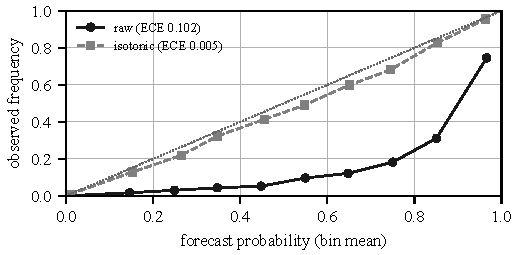
\includegraphics[width=\columnwidth]{fig_rel.pdf}
\caption{Reliability of the forecast probabilities on the unseen test gauges, before and after isotonic recalibration fitted on validation data (bins with at least 50 gauge-days).}
\label{fig:rel}
\end{figure}


The model first warned three days ahead of \WarnThreeXgb\% of the \EvN{} onsets at \EvGauges{} gauges. Climatology and the LSTM simulation did better on this measure, the first because it alarms on most monsoon days, the second because it sees future rain. Lead counts alone reward constant alarms: independent random alarms at the model's rate would warn of \RandWarn\% of onsets on at least one of the three days before them, against \EvXgbWarn\% for the model. Officers act on episodes rather than days, and of the model's \EpN{} alarm episodes \EpFalsePct\% contained no flood window.

Skill was consistent across rivers: over the \PgN{} test gauges with at least one flood window, the median per-gauge balanced accuracy was \PgMed{} (interquartile range \PgQOne--\PgQThree; worst \PgMin). Counting any warning one to three days ahead, the model caught \EvXgbWarn\% of the onsets. The no-flow variant caught more (\EvNoFlowWarn\%), but only because it raised more alarms (\NoFlowAlarms{} per 1,000 gauge-days): in the 500,000-row refits at a common alarm rate, it warned of \MatchWarnNoFlow\% against \MatchWarnAll\% for all inputs.

\subsection{Operating Rules}
\label{sec:rules}
The threshold above maximises balanced accuracy, which favours recall. For committing teams, CSI is the more usual score \cite{Jolliffe2012}, so we also chose thresholds that maximise CSI on the validation years and scored each rule once on the test set (Fig.~\ref{fig:trade}). At its CSI threshold the model alone beat persistence (CSI \McCSI{} against \PeCSI; gain \McPLo--\McPHi). A hybrid rule that raises an alarm whenever the river is already above its level, and otherwise uses the model, added a small further gain (CSI \HyCSI; gain over the model \HyMLo--\HyMHi). It cut the alarms from \MbAlarms{} to \HyAlarms{} per 1,000 gauge-days and raised precision to \HyPrec, but warned of \HyWarn\% of the flood onsets instead of \MbWarn\%. The trade holds along the whole curve: every threshold that warned of at least 80\% of onsets had a CSI of at most \TradeMax. Separate monsoon and dry-season thresholds did not help. The BA threshold therefore suits an early review list, and the hybrid rule suits committing teams.

\begin{figure}[t]
\centering
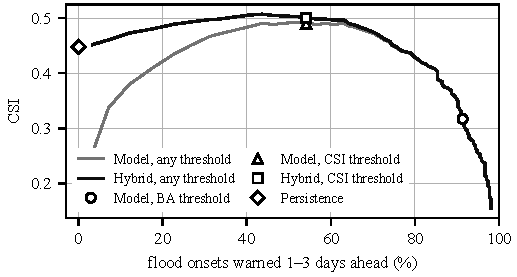
\includegraphics[width=\columnwidth]{fig_trade.pdf}
\caption{Critical success index against the share of flood onsets warned one to three days ahead, on the unseen test gauges, for every threshold. Markers: operating points with thresholds chosen on validation. Hybrid: persistence when the river is above its level, otherwise the model.}
\label{fig:trade}
\end{figure}

\subsection{Where the Forecast Succeeds and Fails}
\textit{Lead day.} The target pools three lead days. Recall fell from \LeadOne\% for a flood on day $t{+}1$ to \LeadThree\% on day $t{+}3$, and from \LeadOneRise\% to \LeadThreeRise\% on rivers still below their level on day $t$.

\textit{Season.} In June to September the model raised \MonAlarms{} alarms per 1,000 gauge-days at a precision of \MonPrec, against \OthAlarms{} and \OthPrec{} in the rest of the year, and \FpMonsoonPct\% of all false alarms fell in the monsoon. Most of these were not near misses: in the median monsoon false alarm the river peaked at \FaRatioMon\% of its flood level over the next three days, and only \NearMissMon\% of them reached 70--100\%.

\textit{Catchment.} Over the \PgGauges{} test gauges with flood windows, per-gauge balanced accuracy rose with catchment area (Spearman $\rho=\RhoArea$, $p=\PArea$), which is consistent with large rivers rising slowly enough for today's flow to describe the next three days. Aridity, mean rainfall and slope showed no relation ($p\ge\PMinOther$).

\section{Discussion and Limitations}
Three findings matter for practice. First, the inputs play different roles. Today's flow carries the overall score, but skill on rivers still below their level owed little to it, so for new floods a meteorological feed matters as much as a gauge feed; when the gauge feed fails, the no-flow variant is a better fallback than climatology. Second, precision is the weak point, mainly in the monsoon, and even the LSTM with future rain reached only \LstmPrec. The hybrid rule raises precision but warns of fewer onsets, so a positive forecast should start an officer's review, and an evacuation needs further evidence. Third, scored on the same rows, a random row split raised balanced accuracy by \SrGapBA{} points and PR-AUC by \SrGapPR{} points, so published Indian flood models can only be compared under the same split.



\iffalse
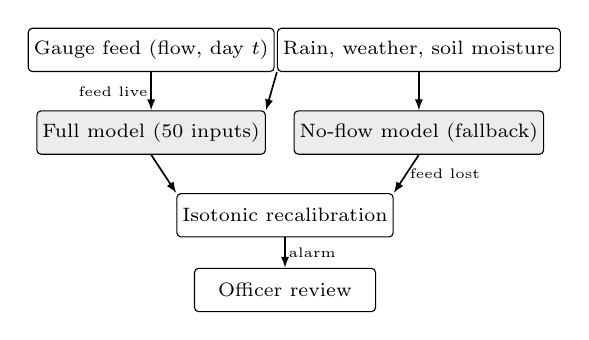
\begin{tikzpicture}[font=\scriptsize,
  box/.style={draw, rounded corners=1.5pt, align=center, minimum height=0.55cm, minimum width=2.3cm, inner sep=2pt},
  arr/.style={-{Latex[length=1.4mm]}, semithick}, lab/.style={font=\tiny, inner sep=1pt}]
\node[box] (g) at (0,0) {Gauge feed (flow, day $t$)};
\node[box] (w) at (3.4,0) {Rain, weather, soil moisture};
\node[box, fill=gray!15] (f) at (0,-1.05) {Full model (\NFeat{} inputs)};
\node[box, fill=gray!15] (n) at (3.4,-1.05) {No-flow model (fallback)};
\node[box] (c) at (1.7,-2.1) {Isotonic recalibration};
\node[box] (o) at (1.7,-3.05) {Officer review};
\draw[arr] (g) -- node[lab, left]{feed live} (f);
\draw[arr] (w) -- (n);
\draw[arr] (w.south west) -- (f.north east);
\draw[arr] (f.south) -- (c.north west);
\draw[arr] (n.south) -- node[lab, right]{feed lost} (c.north east);
\draw[arr] (c) -- node[lab, right]{alarm} (o);
\end{tikzpicture}
\fi

Studies of Indian rivers should therefore hold out gauges and later years, take every threshold from training and validation years, and report precision, alarm rates, below-level skill and calibration.

The study has limits. Almost all test gauge-days fall in \YearsBig, because CAMELS-IND holds few flow records for \YearsSmall. The gauges are in peninsular India only, so skill may not transfer to Himalayan or Brahmaputra rivers. The 95th-percentile level is a statistical proxy, not an official danger level. Inputs available in real time cost little skill, but we used observed rainfall and no rainfall forecast. The LSTM reference was not held out: it was trained on years and, most likely, gauges that overlap our test set, and it sees future rain, so the comparison is indicative only; our own neural baseline was a multilayer perceptron, not a sequence model such as an LSTM trained on the same split. We pool three lead days into one target, and the ablation and protocol models were refitted on a 500,000-row sample (all-input refit \AblAllBA, against \XgbBA{} for the model trained on all rows).

\section{Conclusion}
On CAMELS-IND gauges held out in space and time, a gradient-boosted model forecast three-day exceedance of the 95th-percentile flow with a balanced accuracy of \SplitBAMean{} on average over six gauge splits and \XgbBA{} on the primary split. It scored above persistence, the trend rule and climatology, and it held up over held-out basins (\BasinBAMin--\BasinBAMax). Scored on the same rows, a random row split overstated balanced accuracy by \SrGapBA{} points. Climate indices from training years gave the same skill, and inputs available in real time lowered balanced accuracy by only \RtDiff. On rivers still below their level the skill was lower (\OnXgbBA) and owed little to the flow inputs. At the balanced-accuracy threshold most alarms were false, but a rule that keeps persistence for rivers already above the level and uses the model elsewhere beat persistence on CSI (\HyCSI{} against \PeCSI), though only slightly better than a CSI threshold on the model alone and at the cost of fewer onset warnings. A positive forecast should start an officer's review; the split, the protocol and the two decision rules give a reference against which other forecasters on Indian rivers can be compared.

\section*{Acknowledgment}
The authors thank the CAMELS-IND dataset authors for making their data openly available.
In line with the IEEE policy on AI-generated content, the authors disclose that Claude (Anthropic) was used to help edit and restructure the text of all sections and to draft the experiment and plotting scripts. All experiments use the authors' own software and fixed seeds. The authors checked every number, claim and reference and take full responsibility for the content.

\balance
\begin{thebibliography}{00}
\bibitem{Kratzert2019a} F. Kratzert, D. Klotz, G. Shalev, G. Klambauer, S. Hochreiter, and G. Nearing, ``Towards learning universal, regional, and local hydrological behaviors via machine learning applied to large-sample datasets,'' \textit{Hydrol. Earth Syst. Sci.}, vol. 23, pp. 5089--5110, 2019, doi: 10.5194/hess-23-5089-2019.
\bibitem{Kratzert2019b} F. Kratzert, D. Klotz, M. Herrnegger, A. K. Sampson, S. Hochreiter, and G. S. Nearing, ``Toward improved predictions in ungauged basins: Exploiting the power of machine learning,'' \textit{Water Resour. Res.}, vol. 55, pp. 11344--11354, 2019, doi: 10.1029/2019WR026065.
\bibitem{Nearing2024} G. Nearing \textit{et al.}, ``Global prediction of extreme floods in ungauged watersheds,'' \textit{Nature}, vol. 627, pp. 559--563, 2024, doi: 10.1038/s41586-024-07145-1.
\bibitem{Kapoor2023} S. Kapoor and A. Narayanan, ``Leakage and the reproducibility crisis in machine-learning-based science,'' \textit{Patterns}, vol. 4, no. 9, Art. no. 100804, 2023, doi: 10.1016/j.patter.2023.100804.
\bibitem{Roberts2017} D. R. Roberts \textit{et al.}, ``Cross-validation strategies for data with temporal, spatial, hierarchical, or phylogenetic structure,'' \textit{Ecography}, vol. 40, no. 8, pp. 913--929, 2017, doi: 10.1111/ecog.02881.
\bibitem{Mangukiya2025} N. K. Mangukiya \textit{et al.}, ``CAMELS-IND: Hydrometeorological time series and catchment attributes for 228 catchments in Peninsular India,'' \textit{Earth Syst. Sci. Data}, vol. 17, pp. 461--491, 2025, doi: 10.5194/essd-17-461-2025.
\bibitem{Newman2015} A. J. Newman \textit{et al.}, ``Development of a large-sample watershed-scale hydrometeorological data set for the contiguous USA: Data set characteristics and assessment of regional variability in hydrologic model performance,'' \textit{Hydrol. Earth Syst. Sci.}, vol. 19, pp. 209--223, 2015, doi: 10.5194/hess-19-209-2015.
\bibitem{Addor2017} N. Addor, A. J. Newman, N. Mizukami, and M. P. Clark, ``The CAMELS data set: Catchment attributes and meteorology for large-sample studies,'' \textit{Hydrol. Earth Syst. Sci.}, vol. 21, pp. 5293--5313, 2017, doi: 10.5194/hess-21-5293-2017.
\bibitem{Frame2022} J. M. Frame \textit{et al.}, ``Deep learning rainfall--runoff predictions of extreme events,'' \textit{Hydrol. Earth Syst. Sci.}, vol. 26, pp. 3377--3392, 2022, doi: 10.5194/hess-26-3377-2022.
\bibitem{Kirschstein2024} N. Kirschstein and Y. Sun, ``The merit of river network topology for neural flood forecasting,'' in \textit{Proc. 41st Int. Conf. Mach. Learn. (ICML)}, Vienna, Austria, 2024, vol. 235, pp. 24713--24725.
\bibitem{Alfieri2013} L. Alfieri \textit{et al.}, ``GloFAS -- global ensemble streamflow forecasting and flood early warning,'' \textit{Hydrol. Earth Syst. Sci.}, vol. 17, pp. 1161--1175, 2013, doi: 10.5194/hess-17-1161-2013.
\bibitem{Cloke2009} H. L. Cloke and F. Pappenberger, ``Ensemble flood forecasting: A review,'' \textit{J. Hydrol.}, vol. 375, pp. 613--626, 2009, doi: 10.1016/j.jhydrol.2009.06.005.
\bibitem{Nevo2022} S. Nevo \textit{et al.}, ``Flood forecasting with machine learning models in an operational framework,'' \textit{Hydrol. Earth Syst. Sci.}, vol. 26, no. 15, pp. 4013--4032, 2022, doi: 10.5194/hess-26-4013-2022.
\bibitem{Kuntla2025} S. K. Kuntla and M. Saharia, ``INDOFLOODS: A comprehensive database for flood events in India enhanced with catchment attributes,'' \textit{Bull. Amer. Meteorol. Soc.}, vol. 106, no. 2, pp. E333--E343, 2025, doi: 10.1175/BAMS-D-24-0008.1.
\bibitem{Mosavi2018} A. Mosavi, P. Ozturk, and K.-W. Chau, ``Flood prediction using machine learning models: Literature review,'' \textit{Water}, vol. 10, no. 11, Art. no. 1536, 2018, doi: 10.3390/w10111536.
\bibitem{Saito2015} T. Saito and M. Rehmsmeier, ``The precision-recall plot is more informative than the ROC plot when evaluating binary classifiers on imbalanced datasets,'' \textit{PLoS ONE}, vol. 10, no. 3, Art. no. e0118432, 2015, doi: 10.1371/journal.pone.0118432.
\bibitem{Brier1950} G. W. Brier, ``Verification of forecasts expressed in terms of probability,'' \textit{Mon. Weather Rev.}, vol. 78, no. 1, pp. 1--3, 1950.
\bibitem{Chen2016} T. Chen and C. Guestrin, ``XGBoost: A scalable tree boosting system,'' in \textit{Proc. 22nd ACM SIGKDD Int. Conf. Knowl. Discov. Data Min.}, San Francisco, CA, USA, 2016, pp. 785--794, doi: 10.1145/2939672.2939785.
\bibitem{Naeini2015} M. P. Naeini, G. F. Cooper, and M. Hauskrecht, ``Obtaining well calibrated probabilities using Bayesian binning,'' in \textit{Proc. 29th AAAI Conf. Artif. Intell.}, Austin, TX, USA, 2015, pp. 2901--2907.
\bibitem{Jolliffe2012} I. T. Jolliffe and D. B. Stephenson, Eds., \textit{Forecast Verification: A Practitioner's Guide in Atmospheric Science}, 2nd ed. Chichester, U.K.: Wiley, 2012.
\bibitem{Zadrozny2002} B. Zadrozny and C. Elkan, ``Transforming classifier scores into accurate multiclass probability estimates,'' in \textit{Proc. 8th ACM SIGKDD Int. Conf. Knowl. Discov. Data Min.}, Edmonton, AB, Canada, 2002, pp. 694--699.
\end{thebibliography}

\end{document}
